\chapter{Wyniki eksperymentów}
\label{c5}

\section{Wstęp}
\label{c51}
W poniższym rozdziale opisano przebieg przeprowadzonych eksperymentów oraz przedstawiono uzyskane wyniki wraz z ich interpretacją. Algorytmy testowane były na tych samych zbiorach danych. Tworzenie tych zbiorów odbywało się z wykorzystaniem generatora przyjmującego jako parametry liczbę transakcji (np. 10 tys., 100 tys.), średnią liczbę elementów w transakcji (np. 6), liczbę wzorców do odkrycia (np. 500), średni rozmiar wzorców częstych do odkrycia (np. 3), liczbę różnych elementów występujących w transakcjach (np. 1000, 10000) oraz nazwę pliku wyjściowego. Wygenerowany plik jest importowany do bazy danych, do której odwołuje się aplikacja podczas wykonywania algorytmów. Dane w bazie składowane są w jednej tabeli w postaci par \((id transakcji, id elementu)\). Dlatego też po odczycie tej tabeli składane są transakcje wykorzystywane w dalszym przetwarzaniu. Zbiór zapytań \(DMQ\) generowany był przed rozpoczęciem przetwarzania. Liczba transakcji obejmująca każde zapytanie \(dmq_i\) wynosi \(|T|/|DMQ|\), gdzie \(|T|\) - liczba wszystkich transakcji, \(|DMQ|\) - liczba wszystkich zapytań eksploracyjnych. 

\section{Opis infrastruktury}
\label{c52}
Algorytmy napisane zostały w języku Java, z wykorzystaniem narzędzia Maven oraz środowiska programistycznego Eclipse. Dane testowe generowane były za pomocą generatora GEN (\cite{AgrawalGEN}), a następnie wczytywane do bazy PostgreSQL, z której korzystała aplikacja. Testy przeprowadzone zostały na komputerze HP Envy 14 Notebook PC, z procesorem Intel Core i5-2410M 2x2.30GHz oraz 8GB pamięci RAM, pracującym pod kontrola systemu operacyjnego Microsoft Windows 7. 

\section{Wyniki}
\label{c53}
Poniżej zaprezentowano wyniki eksperymentów. Wszystkie uwzględnione czasy są średnią 4 dokonanych pomiarów dla dokładnie tych samych parametrów. Badania przeprowadzono dla dwóch zapytań eksploracyjnych z różnym poziomem nakładania się danych. Oba zapytania wykorzystywały ten sam próg wsparcia, mimo że nie jest to wymaganiem algorytmu. Jest to podyktowane chęcią możliwości lepszego zaobserwowania różnic w działaniu algorytmów niezależnie od wykorzystywanych progów dla poszczególnych zapytań. Algorytmy uwzględniane w wynikach to Common Counting z wykorzystaniem drzew prefiksowych (CCP), Common Candidate z wykorzystaniem drzew prefiksowych (CCTP) oraz sekwencyjnie wykonywana adaptacja algorytmu Apriori (SEQ) zgodna z tą zastosowaną wewnątrz CCP i CCTP.

Zbiór danych 1. Parametry generatora dla drugiego zbioru danych przedstawia tabela \ref{table:firstDataSetParams}.
\begin{table}[h]
\begin{center}
	\begin{tabular}{| l | c |}
		\hline
		liczba transakcji & 100000 \\ \hline
		średnia liczba elementów w transakcji & 8 \\ \hline
		liczba różnych elementów & 1000 \\ \hline
		liczba wzorców (zbiorów częstych) & 1500 \\ \hline
		średnia liczba elementów we wzorcu & 4 \\ 
		\hline
	\end{tabular}
\end{center}
\caption{Parametry generatora dla pierwszego testowego zbioru transakcji.}
\label{table:firstDataSetParams}
\end{table}

\begin{figure}[h]
	\centering
	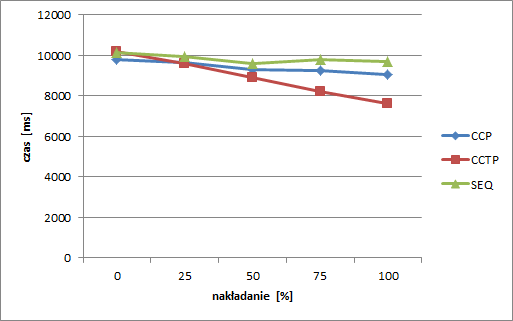
\includegraphics[width=0.8\linewidth]{figures/chart_100_2}
	\caption{Wykres dla pierwszego zbioru danych dla dwóch zapytań \(dmq\) z różnym stopniem nakładania się i \(minsup = 2\%\)}
	\label{fig:chart_100_2}
\end{figure}

Na wykresie \ref{fig:chart_100_2} zestawione czasy trwania poszczególnych algorytmów wykonywanych na pierwszym zbiorze danych z różnymi stopniami nakładania się. Przyjęta wartość \(minsup\) dla wszystkich zapytań wynosiła 2\%. Jak widać na wykresie w przypadku braku nakładania się zapytań uzyskane czasy były do siebie bardzo zbliżone. Wraz ze wzrostem stopnia nakładania się uwidaczniały się różnice w czasach wykonania algorytmów. Wykonanie sekwencyjne cały czas utrzymywało się na niemalże takim samym poziomie. Jest to związane z podobną liczbą operacji wykonywaną w trakcie działania algorytmu. W przypadku CCP i CCTP wraz ze wzrostem nakładania zwiększała się współbieżność. W przypadku CCTP skrócenie czasu następuje szybciej niż ma to miejsce dla CCP. Jednakże dla CCP także zaobserwowany został stały spadek czasu wykonania. Można powiedzieć, że dla tego przypadku algorytm CCTP okazał się zdecydowanie najlepszy, a także zastosowanie CCP zamiast SEQ skutkowało krótszym czasem udzielenie odpowiedzi na zadane zapytania eksploracyjne.

\begin{figure}[h]
	\centering
	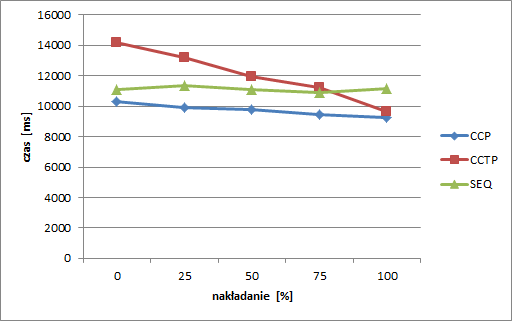
\includegraphics[width=0.8\linewidth]{figures/chart_100_1}
	\caption{Wykres dla pierwszego zbioru danych dla dwóch zapytań \(dmq\) z różnym stopniem nakładania się i \(minsup = 1\%\)}
	\label{fig:chart_100_1}
\end{figure}
Drugi rozważany przypadek na pierwszym zbiorze danych został przedstawiony na wykresie~\ref{fig:chart_100_1}. Przyjęto \(minsup\) ma poziomie 1\%. Mniejsza wartość progu minimalnego wsparcia przekłada się na większą liczbę zbiorów częstych odkrywanych w trakcie wykonań algorytmów, stąd też wydłużenie czasów wykonania. W przypadku wykonania sekwencyjnego po raz kolejny widoczny jest brak wpływu nakładania się zapytań eksploracyjnych. Podobnie jak w pierwszym analizowanym przykładzie zachowuje się algorytm Common Counting. Widoczne jest skracanie czasu wykonania wraz ze wzrostem nakładania się zapytań. Jest to zależność liniowa i mimo, że przyspieszenie nie jest bardzo znaczące, to po raz kolejny CCP działa szybciej niż SEQ. Ciekawa sytuacja została zaobserwowana dla Common Candidate Tree. Znowu widoczny jest stały, liniowy spadek czasu wykonania, ale tym razem algorytm dla większości rozważanych przypadków nakładania się \(dmq\) działa wolniej. Jest to zapewne spowodowane koniecznością sprawdzania kolejności (i sortowania jeśli jest to niezbędne) elementów w danym wierzchołku (problem ten opisany został w \ref{c46}). Nie było to widoczne dla \(minsup = 2\%\) ze względu na mniejszą liczbę zbiorów częstych na każdym poziomie drzewa, co ma bezpośrednie przełożenie na liczbę kandydatów na kolejnym poziomie, a więc liczbę dodawanych do drzewa wierzchołków. Mimo to dla znaczącego nakładania się obserwowany jest zysk względem SEQ. 


Zbiór danych 2. Parametry generatora dla drugiego zbioru danych przedstawia tabela \ref{table:secondDataSetParams}. 
\begin{table}[h]
	\begin{center}
		\begin{tabular}{| l | c |}
			\hline
			liczba transakcji & 50000 \\ \hline
			średnia liczba elementów w transakcji & 8 \\ \hline
			liczba różnych elementów & 1000 \\ \hline
			liczba wzorców (zbiorów częstych) & 1000 \\ \hline
			średnia liczba elementów we wzorcu & 4 \\ 
			\hline
		\end{tabular}
	\end{center}
	\caption{Parametry generatora dla drugiego testowego zbioru transakcji.}
	\label{table:secondDataSetParams}
\end{table}

\begin{figure}[h]
	\centering
	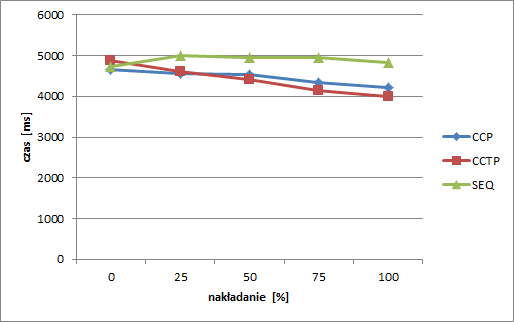
\includegraphics[width=0.8\linewidth]{figures/chart_50_2}
	\caption{Wykres dla drugiego zbioru danych dla dwóch zapytań \(dmq\) z różnym stopnieniem nakładania się i \(minsup = 2\%\)}
	\label{fig:chart_50_2}
\end{figure}
Wykres \ref{fig:chart_50_2} obrazuje czasy wykonania algorytmów dla mniejszego z wygenerowanych zbiorów danych, na których przeprowadzane były testy. Podobnie jak miało to miejsce w uprzednio opisanych przypadkach czasy wykonania SEQ są niemalże liniowe. Zaobserwowane drobne różnice wynikają prawdopodobnie z tego, że zapytania odnoszą się do różnych podzbiorów zbioru danych, a także wpływem chwilowych różnic w działaniu środowiska testowego. Patrząc na wyniki uzyskane przez CCP o CCTP okazuje się, że są one bardzo zbliżone. Po raz kolejny czas wykonania maleje szybciej dla Common Candidate Tree niż dla Common Counting. Jednakże dla przyjętych dla tej obserwacji parametrów ciężko jednoznacznie wskazać algorytm lepszy, aczkolwiek oba są szybsze od algorytmu sekwencyjnego. 

\begin{figure}[h]
	\centering
	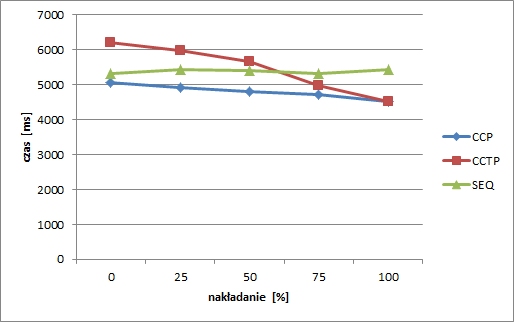
\includegraphics[width=0.8\linewidth]{figures/chart_50_1}
	\caption{Wykres dla drugiego zbioru danych dla dwóch zapytań \(dmq\) z różnym stopnieniem nakładania się i \(minsup = 1\%\)}
	\label{fig:chart_50_1}
\end{figure}
Na wykresie \ref{fig:chart_50_1} zaprezentowano wyniki uzyskane dla drugiego zbioru danych przy założeniu, że próg minimalnego wsparcia wynosi \(1\%\). Potwierdza on niezależność wykonania sekwencyjnego względem stopnia nakładania się zapytań \(dmq_i\). Obserwowane rezultaty dla CCP i CCTP przypominają te uzyskane dla pierwszego zbioru danych i \(minsup = 1\%\). Widoczny jest dłuższy czas wykonania CCTP, w stosunku do SEQ i CCP, dla zapytań nie nakładających się lub małego stopnia nakładania. Powodem jest tak jak poprzednio konieczność wykonywania większej liczby sprawdzeń kolejności elementów w wierzchołku (i ewentualnych sortowań). Nie zmienia to faktu, że widoczny jest stały spadek czasu wykonania wraz ze wzrostem współbieżności. Z kolei Common Counting potwierdza swoją przewagę nad wykonaniem sekwencyjnym oraz fakt, że zwiększanie stopnia nakładania się zapytań działa na rzecz skrócenia (proporcjonalnie do zwiększania się nakładania) przetwarzania \(DMQ\) tym algorytmem. 

\section{Porównanie CCP i CCTP z CC i CCT}
\label{c54}
Powołując się na wyniki uzyskane w \cite{WojciechowskiCC} oraz \cite{WojciechowskiCCT} można stwierdzić, że zastosowanie Common Counting wykorzystującego struktury prefiksowe daje podobny efekt jak w przypadku drzew haszowych. Efektem tym jest stały wzrost szybkości przetwarzania proporcjonalny do stopnia nakładania się danych. Nieco inaczej rzecz ma się dla Common Candidate Tree. Po zmianie drzewa haszowego na prefiksowe dla algorytmu nadal obserwowany jest liniowy (szybszy niż dla CC) spadek czasu wykonania. Niestety w przypadkach gdy na każdym poziomie drzewa generowanych jest dużo kandydatów (np. stosunkowo małe \(minsup\)) i nie występuje duże nakładanie się zapytań, to algorytm ten traci swoją przewagę. Jest to przewaga CCT (\cite{WojciechowskiCCT}), gdyż dla drzewa haszowego kolejność dodawania wierzchołków nie ma wpływu na przetwarzanie.

